% Chapter 5

\chapter{Model Based Reinforcement Learning} % Main chapter title

\label{Chapter5} 
In this chapter we focus on Model Based approach, explaining how in works theoretically, why is useful and how could use it to create better agents. Then we present some  significant proposal from the literature and lastly we introduce the model used for this thesis. 


% Method name
\newcommand{\method}{PlaNet}
\newcommand{\fullmethod}{Deep Planning Network }
\newcommand{\Foruno}{\\  $\mathbf{\textbf{for } }$  }
\newcommand{\Fordue}{\\ \tab{} $\mathbf{\textbf{for } }$  }
\newcommand{\Fortre}{\\ \tab{} \tab{} $\mathbf{\textbf{for } }$  }
%\newcommand\tab[1][1cm]{\hspace*{#1}}
%\newcommand\Doubletab[1][2cm]{\hspace*{#1}}

\section{Model Based Reinforcement Learning}
% intro presa da https://arxiv.org/pdf/1903.11981.pdf

As we said in chapter \ref{Chapter3} in the reinforcement setting, there is an environment in a specific state $s_t$ that receives an action $a_t$ from an agent. 
After receiving this action, the environment update its state using the transition probability function $s_{t+1} = f\left(s_{t}, a_{t}\right)$
and calculates also the correspective reward $r_{t+1}=r\left(s_{t}, a_{t}\right).$
The agent takes the new observation from the environment and uses that to choose the next action to take $a_t=\pi(a_t|o_t)$.
Recall that in an MDP on observation correspond to the state, so $o_t = s_t$, while in an POMDP the observation is derivative of the state, so $o_t=o(s_t)$.

In the model-free setting, the agent will learn a policy that returns the best action directly to take in that state in order to maximize the expected cumulative reward.
In the model-based setting, instead, the agent will learn to model the dynamics of the environment (forward model) by approximating the transition function and the reward function.
So in case of MDP the model could be:
$ s_{t+1} = f_\theta (s_t,a_t).$
Instead if the environment is a POMDP the model need to use also the old observation and actions, in order to predict a new one.
$ o_{t+1} = f_\theta(o_0,a_0,...,o_t, a_t)$

Once the agent is able to approximate the environment in its head, it is also able to  simulate actions and predicts the possible consequences.

To be more specific, the agent plan a sequence of H (that stands for Horizon) actions $ \left\{ a_{t},\ldots, a_{t+H}\right\}$, and then unroll the learned model H step into the future based on those actions.
Now the agent can compute the objective function. 
$ G\left(a_{t}, \ldots, a_{t+H}\right) =\mathbb{E}\left[\sum_{\tau=t}^{t+H} r\left(o_{\tau}, a_{\tau}\right)\right] $ to evaluate the current plan and performs some sort of optimization to find the best possible plan (often a genetic algorithm is used to this purpose)
$ a_{t}, \ldots, a_{t+H} =\arg \max G\left(a_{t}, \ldots, a_{t+H}\right) $.
This process is called  \textbf{trajectory optimization}.


\section{Planet}
Planet is a new algorithm published in 2019 from the research team in Google AI \cite{hafner2019learning}.
In this paper, the agent is able to learn environment dynamics only through the observation and then can use this model to plan what action to take for each step.
In order to achieve this task, the agent must solve three problems:

\begin{enumerate}
\item understanding the observation: capture the useful information contained in each frame and maintain them in memory
\item understanding the environment dynamics: be able to predict the next observation and the next reward having only the current observation and the current action as input
\item using its prediction to plan what action to take.
\end{enumerate}

\subsection{RSSM}
Since the planning requires a considerable amount of predictions at every time step, the researchers decided to work in latent space.
In other words, they do not use the entire frame to predict the next one, but they encode all the information in a vector obtained from neural networks, called latent vector. 
This advantage in terms of computational cost leads to a disadvantage for the agent that now has two jobs: first, it has to build a visual understanding of the environment and second, it has to find a way to solve the task.
To be more specific, they use a convolutional neural network to capture all the spatial information from the image, and a GRU network  (a simplified version of LSTM) to capture the temporal information across different time steps.
Then they use both information to create the latent vector.

Now it is time to enter in technical details:
We now considering sequences like $\left\{o_{t}, a_{t}, r_{t}\right\}_{t=1}^{T}$ where the index $t$ is used for the time step, $o_t$ is the environment observation for the current time step, $a_t$ and $r_t$ the current action and reward.
The Planet model is composed of three sub models:
\begin{align*}
\text { Transition model: } & s_{t} \sim p\left(s_{t} \mid s_{t-1}, a_{t-1}\right) \\
\text { Observation model: } & o_{t} \sim p\left(o_{t} \mid s_{t}\right) \\
\text { Reward model: } & r_{t} \sim p\left(r_{t} \mid s_{t}\right)
\end{align*}
The transition model has the job of produce the current latent state by using the previous latent state and the current action.
Then the observation model and the reward model will use it to reconstruct the observation and predict the reward obtained by the execution of $a_{t}$  in $s_{t}$. 

The \textbf{observation model} is Gaussian with a mean parameterized by a deconvolutional neural network and identity covariance.
The \textbf{reward model} is a scalar Gaussian with a mean parameterized by a feed-forward neural network and unit variance.
In both cases, the loss is calculated through mean square error.
The \textbf{transition model} can be viewed as a sequential VAE that is a convolutional variational autoencoder that receive in input an observation $o_t$ and an action $a_t$.
The aim of the encoder is to learn an approximation of the state posterior $q\left( s_{1:T} \mid o_{1:T}, a_{1:T}   \right) $ from past observation and actions. 
This state posterior will contain all the useful information about the current state to allow the decoder (introduced above as the observation model) to uses this state $s_t$ to reconstruct the observation $o_t$ completely.
When it produces the current posterior state, it needs to use also the information of the precedent state that is served as input in addition to the observation and action, and this is why it is called \textit{recurrent} VAE.
So the transition model approximate the true state posterior with $\prod_{t=1}^{T} q\left(s_{t} \mid s_{t-1}, a_{t-1}, o_{t}\right)$.
We can find the true parameters of this Gaussian at training time because we have all the information necessary to calculate the loss value througth mean squared error. 
Another important point is that at training time we can always sample a batch of transitions from the experience replay and  provide the current observation for each time step. 
At inference time instead, we only have the observation for the current step, but if we want to predict the posterior states of different steps in the future, we cannot provide the respective observation.

Intuitively if we ask the model to predict the next observations, it cannot require it as input.
For this reason we use this model at training time to find the correct parameter of the posterior state and in inference time we use another model that not use the information about the current observation $o_t$ but  it only require $s_{t-1}$ and $a_{t-1}$ $p(s_t | s_{t-1}, a_{t-1})$.
This new model $p$ is trained to stay close to $q$ via kl-divergence.
$KL\left[ q\left(s_{t} \mid s_{t-1}, a_{t-1}, o_{t}\right) || p\left(s_{t} \mid s_{t-1}, a_{t-1}\right)  \right]$.

Unfortunately, the only $s_{t-1}$ is not enough to maintain in memory all the useful information.
The form of stochastic transition, in fact, not able to maintain information across multiple steps.
For this reason, they also provide the model with a sequence of activation vectors $\left( h_t \right) ^{T}_{t=1}$ from a GRU network.
Combining these two methods, they create a new model called \textbf{Recurrent State-Space Model (RSSM)}.
In RSSM, the internal state is composed of two parts: a stochastic one named $s_t$ (sampled from a Gaussian) and a determinist part $h_t$ (sampled from GRU).
The final model is similar to the previous one:
\begin{align*}
\text { Deterministic state model: } & h_{t} = f\left(h_{t-1} , s_{t-1}, a_{t-1}\right) \\
\text { Stocastic state  model: } & s_{t} \sim p\left(s_{t} \mid h_{t}\right)  \text {*}\\
\text { Observation model: } & o_{t} \sim p\left(o_{t} \mid h_{t}, s_{t}\right) \\
\text { Reward model: } & r_{t} \sim p\left(r_{t} \mid h_{t}, s_{t}\right)\\
\text{*the information over action is already encoded in h}
\end{align*}
Now at inference time, the model can rely only on $h_t$.

Before moving on to the next paragraph, I left a quick visual recap of the Planet model.

\begin{figure}[H]
\centering
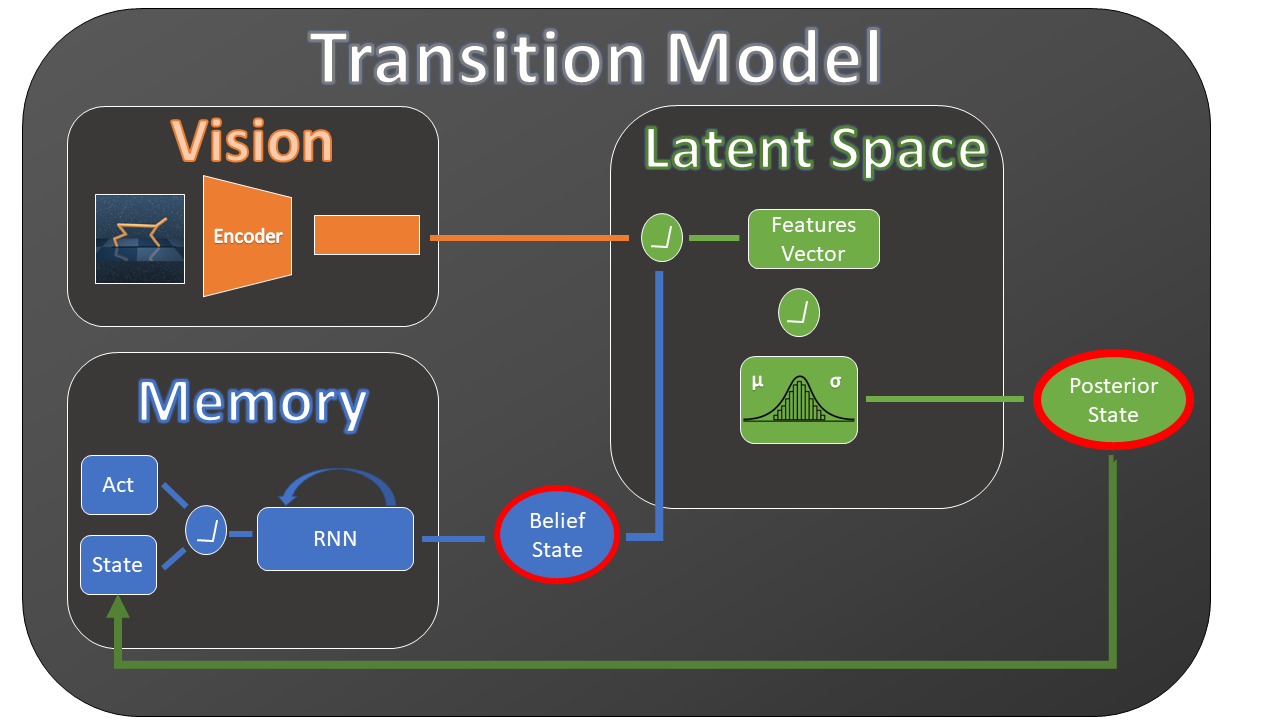
\includegraphics[width=1.\textwidth, height=.4\textheight]{pictures/planet_schema}
\caption{ The transition model at inference time. The current frame is encoded and the RNN produces the current Belief State encoding the current action and the previous posterior state. The current encoded observation and the Belief State are combined to produce the Features Vector from where the posterior Gaussian parameters are produced. In the last step, the current Posterior state is sampled from the Gaussian.}
\end{figure}

\begin{figure}[H]
\centering
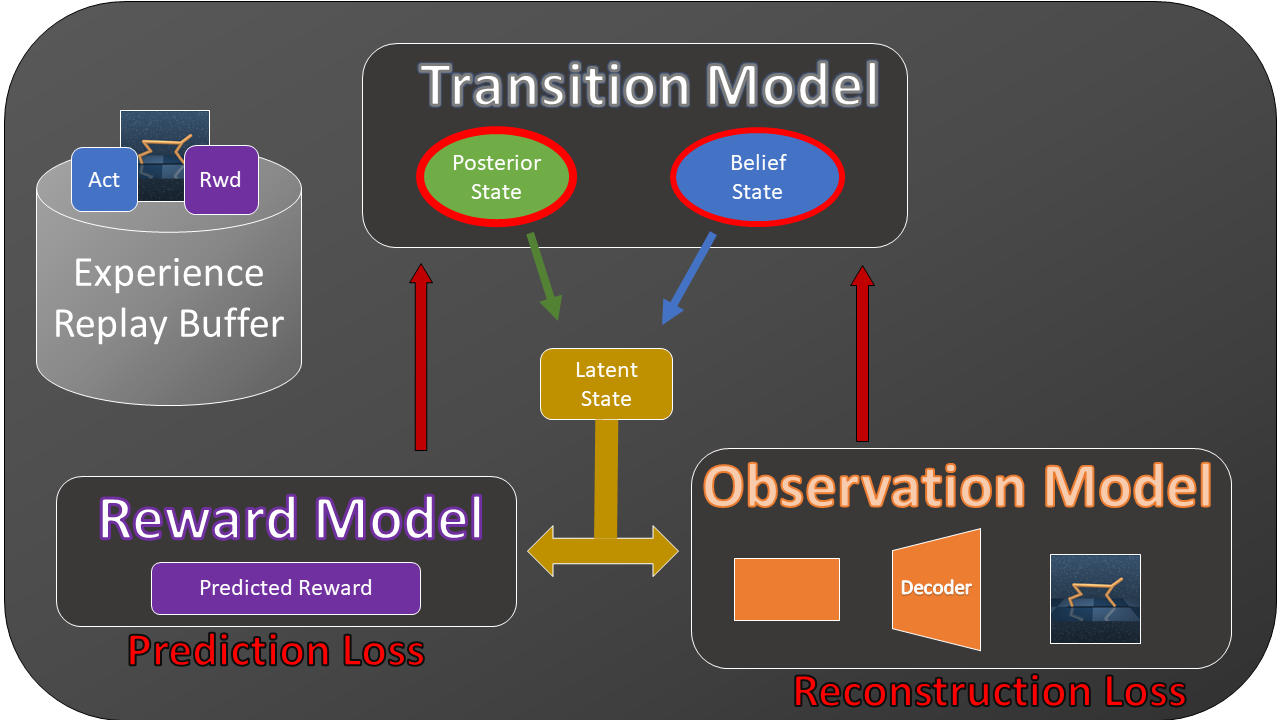
\includegraphics[width=1.\textwidth, height=.4\textheight]{pictures/planet_loss}
\caption{ The current Latent State is produced by the combination of both Belief State and Posterior State. This Latent State is then used by the Reward Model to predict the reward and by the Observation Model to reconstruct the current observation. With these two results we can calculate the mean squared error (by sampling the original result from the buffer) and backpropagate the loss to train the transition model. }
\end{figure}

\begin{figure}[H]
\centering
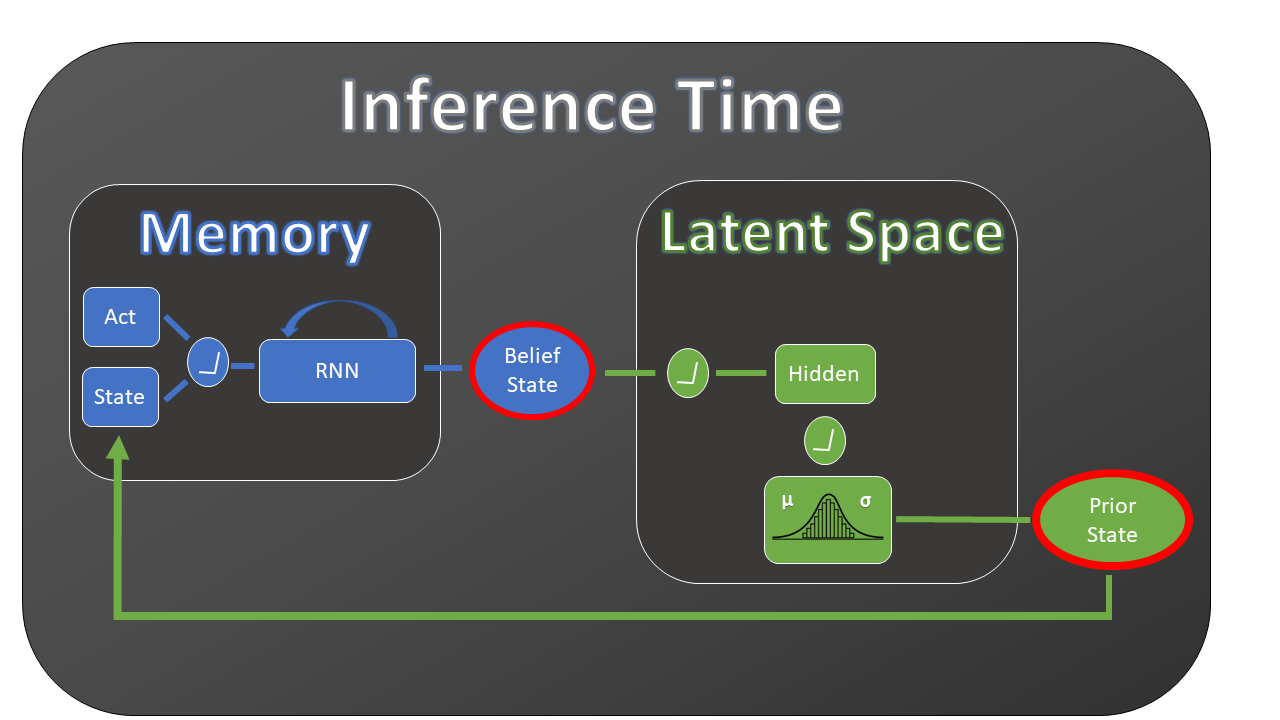
\includegraphics[width=1.\textwidth, height=.4\textheight]{pictures/planet_inference}
\caption{ At inference time we have no more the experience replay buffer that provide us the observation for each step. We only have the observation for the current step provided by the environment and we have to predict the next for many steps ahead.}
\end{figure}
\begin{figure}[H]
\centering
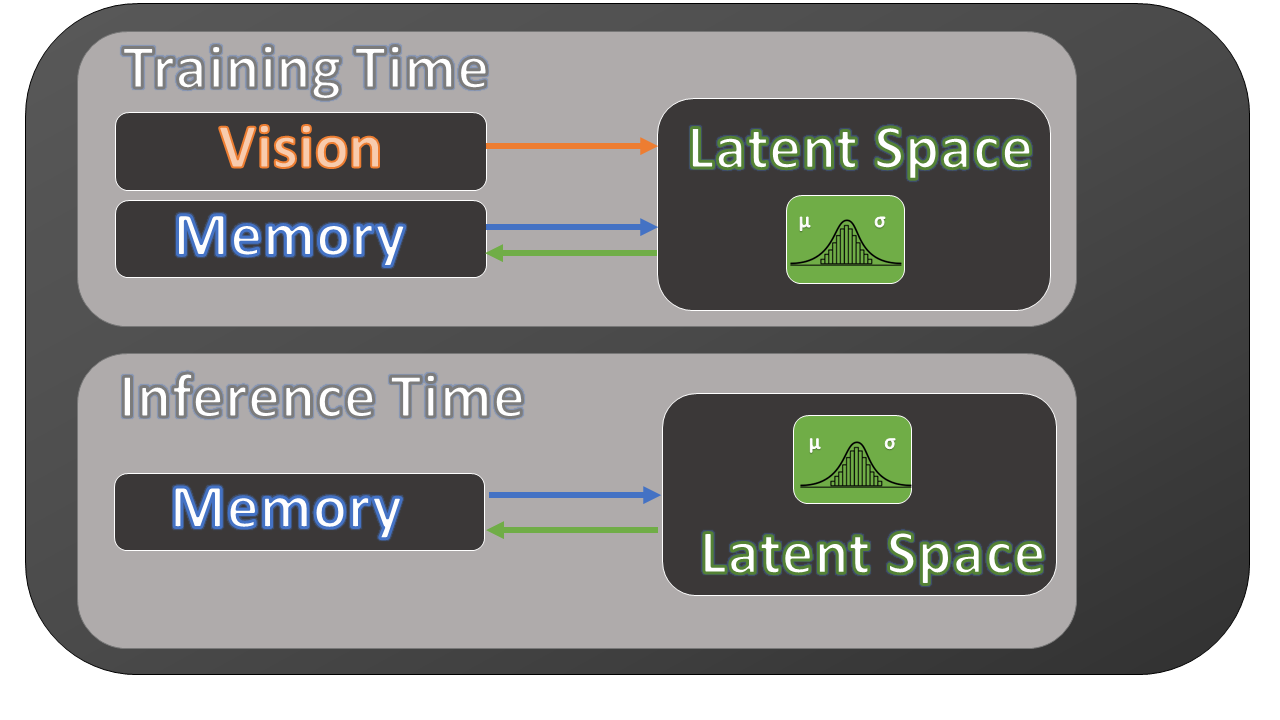
\includegraphics[width=1.\textwidth, height=.4\textheight]{pictures/planet_train_infer}
\caption{ We can reuse the Memory model (RNN) used for the transition model at training time but we need to retrain the Gaussian model. We need a way to obtain the same parameters  used by the model at training time. }
\end{figure}
\begin{figure}[H]
\centering
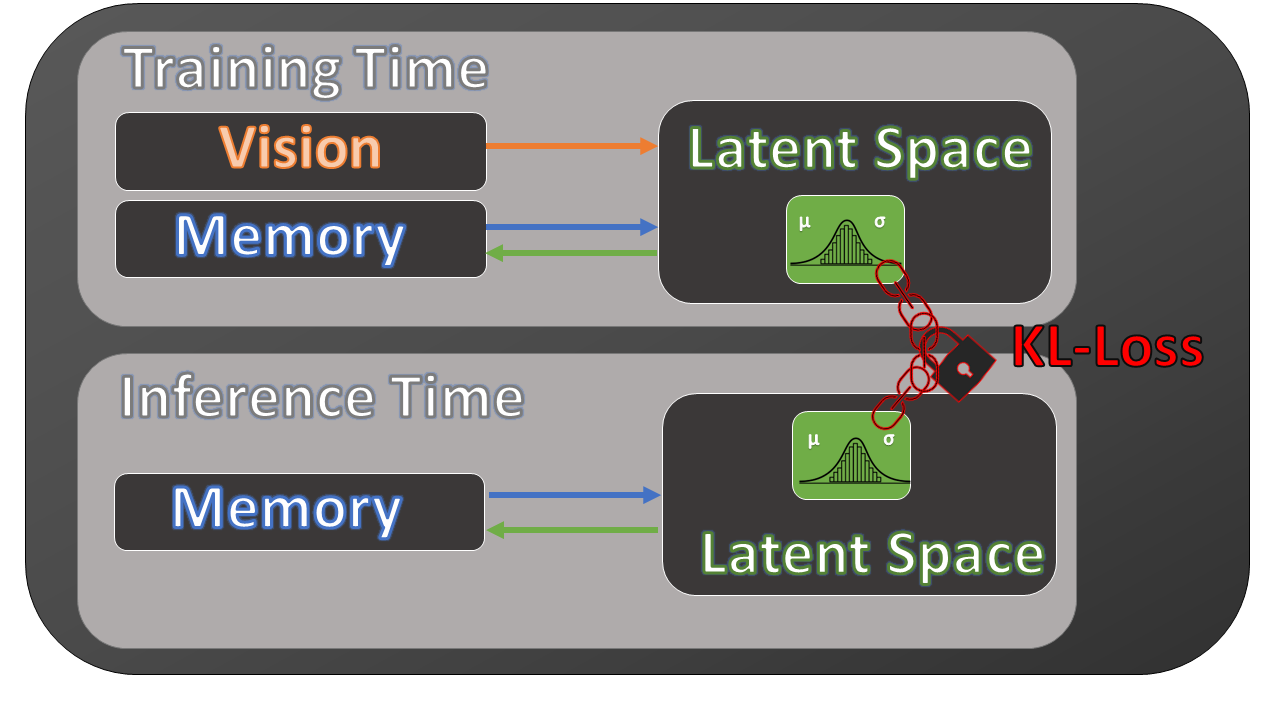
\includegraphics[width=1.\textwidth, height=.4\textheight]{pictures/kl_loss_chain}
\caption{ The loss indicates how much information we lost by approximate the Gaussian produced at training time with the one used at inference time. }
\end{figure}


\subsection{Planning}
Now it's time to use the model for planning. 
Even if the model that predicts the future is robust, a perfect prediction over the entire episode is unrealistic. 
The more we try to predict in the future, the more the prediction error will accumulate, and the more the prediction will diverge to reality.
For this reason, the planning is computed over a short horizon $H$.
They used the Cross-Entropy Method to perform trajectory optimization. It is a robust method and is proved to be capable of solving all the tested environments when true dynamics are given.
Initially, the actions vector, that contains all the actions from the current time step $t$ to the planning horizon $H$, is sampled from a Gaussian with zero mean and unit variance $a_{t: t+H} \sim \operatorname{Normal}\left(\mu_{t: t+H}, \sigma_{t: t+H}^{2} \right)$.
For each generation, $J$ candidates action vectors are sampled and evaluated using the transition model and the reward model.
The evaluation is base on how much reward is produced over the time steps.
For each generation, the parameters update of the Gaussian is calculated over the top k elements of the candidates' population.
Even if the planner has produced a plan over H time steps when the first action is executed, and the new observation is received, the planning process is replicated and adapted to the latest information.
In other words, the planning is computed at every step, and only the first planned action is used. 
It is still necessary to planning over a horizon longer than one because that will lead to local optima.

\section{Cross Entropy Method}
%https://arxiv.org/pdf/1810.01222.pdf

The Cross-entropy (CE) method is an EDA (Estimation of Distribution Algorithms) used in many optimization problems of the form:
$$w^{*}=\arg \max _{w} S(w)$$
where w is a set o weight, and S is a generic objective function of w. 
The EDA is a specific family of Genetic Algorithms that
does not work with a single solution but distributions of possible solutions represented with a covariance matrix $ \Sigma $.
This covariance matrix is used to defines a multivariate Gaussian function and for sampling the population for the next iteration.
Iterations after iterations, the ellipsoid defined by $\Sigma$ is moved to the top part of the hill corresponding to the local optimum $\theta^*$.
A each time step the entire population is sampled from the current parameters of the distributions. 
Next So all the new individuals are evaluated according to the problem-dependent fitness function $(f_i)_{i=1,...,\lambda}$.
Then the top $K_e$ individuals $(z_i)_{i=1,...,K_e}$ (called \textbf{elites} or \textbf{candidates}) are used to update the distribution parameters (the new mean and variance are calculated over the elites).

\begin{align*} 
\mu_{n e w} &=\sum_{i=1}^{K_{e}} \lambda_{i} z_{i} \\ \Sigma_{n e w} &=\sum_{i=1}^{K_{e}} \lambda_{i}\left(z_{i}-\mu_{o l d}\right)\left(z_{i}-\mu_{o l d}\right)^{T}+\epsilon \mathcal{I}, 
\end{align*}

Notice that $(\lambda_i)_{i=1,...,K_e}$ are weights assigned to each individual (a common choice is $\lambda_i = \frac{1}{K_e}$.
Usually some extra variance $\epsilon$ is added in order to prevent premature convergence.
To be more specific some Gaussian noise is added to each individual $x_i$ that is sampled from the current covariance matrix $\Sigma$.

\begin{algorithm}[h!]
\textbf{Input:}
\begin{tabular}[t]{l @{\hspace{.5em}} l}
$H$ & Planning horizon distance \\
$I$ & Optimization iterations \\
$J$ & Candidates per iteration \\
$K$ & Number of top candidates to fit \\
\end{tabular}%
\begin{tabular}[t]{l @{\hspace{.5em}} l}
$q(s_t|o_{\leq t},a_{<t})$ & Current state belief \\
$p(s_t|s_{t-1},a_{t-1})$ & Transition model \\
$p(r_t|s_t)$ & Reward model \\
\end{tabular}% 
\\ Initialize factorized belief over action sequences $q\left(a_{t: t+H}\right) \leftarrow \operatorname{Normal}(0, \mathbb{I})$. \;
\Foruno{optimization iteration $i=1..I$}{
  \\\tab{ \textit{// Evaluate $J$ action sequences from the current belief.}}
  \Fordue{candidate action sequence $j=1..J$}{
     \\\Doubletab{ $a^{(j)}_{t:t+H}\sim q(a_{t:t+H})$ \;}
     \\\Doubletab{ $s^{(j)}_{t:t+H+1}\sim
        q(s_t|o_{1:t},a_{1:t-1})
        \prod_{\tau=t+1}^{t+H+1}p(s_\tau|s_{\tau-1},a^{(j)}_{\tau-1})$ \;}
      \\\Doubletab{ $R^{(j)}=\sum_{\tau=t+1}^{t+H+1}E{p(r_\tau|s^{(j)}_\tau)}$ \;}
  }
  \\\tab{\textit{//Re-fit belief to the $K$ best action sequences}.}
  \\\tab{$\mathcal{K}\leftarrow\mathrm{argsort}(\{R^{(j)}\}_{j=1}^J)_{1:K}$ \;}
  \\\tab{$\mu_{t:t+H}=\frac{1}{K}\sum_{k\in\mathcal{K}} a_{t:t+H}^{(k)}, \quad
  \sigma_{t:t+H}=\frac{1}{K-1}\sum_{k\in\mathcal{K}}|a_{t:t+H}^{(k)}-\mu_{t:t+H}|$. \;}
  \\\tab{$q(a_{t:t+H})\leftarrow\operatorname{Normal}(\mu_{t:t+H},\sigma_{t:t+H}^2\mathbb{I})$ \;}
}
\\\Return{first action mean $\mu_t$.}
\caption{Latent planning with CEM}
\label{alg:planner}
\end{algorithm}

\subsection{Algorithm}
Finally, we have all the information to describe the entire flow of the Planet algorithm.
Initially, some random episodes ( every action is chosen randomly) are executed in order to collect some data in the experience replay buffer.
Then the main training loop, which is composed of two procedures called model fitting and data collection, can begin.
\textbf{The model fitting procedure} consists of sampling sequence chunks from the buffer experience and train the model.
\textbf{The data collection procedure} consists of using the model to solve an episode and collect new data. 
Since the aim of this procedure is not to solve the environment but collect new data, random Gaussian noise is added over the action before it is executed to have a better exploration of the environment.
This noise is not used when we want to use/evaluate the model.





This iterative approach allows the model to collect also the data that is not obtainable from the random init episodes.



\begin{algorithm}
\textbf{Input:}
{\\\hspace{-3.6em}\small
\begin{tabular}[t]{l @{\hspace{.5em}} l}%
$R$ & Action repeat \\
$S$ & Seed episodes \\
$C$ & Collect interval \\
$B$ & Batch size \\
$L$ & Chunk length \\
$\alpha$ & Learning rate \\
\end{tabular}\hspace{-0.5em}%
\begin{tabular}[t]{l @{\hspace{.5em}} l}%
$p(s_t|s_{t-1},a_{t-1})$ & Transition model \\
$p(o_t|s_t)$ & Observation model \\
$p(r_t|s_t)$ & Reward model \\
$q(s_t|o_{\leq t},a_{<t})$ & Encoder \\
$p(\epsilon)$ & Exploration noise \\
\end{tabular}%
}
\\
\\Initialize dataset $\mathcal{D}$ with $S$ random seed episodes.
\\Initialize model parameters $\theta$ randomly. \;
\\
\textbf{while}{(not converged)}{
	 \\
	\tab{// Model fitting}
	\Fordue{update step $s=1..C$}{ 
    \\\Doubletab{Draw sequence chunks $\{(o_t,a_t,r_t)_{t=k}^{L+k}\}_{i=1}^B\sim\mathcal{D}$ uniformly at random} \Doubletab{ from the dataset.}
   \\\Doubletab{ Compute loss $\mathcal{L}(\theta)$ . \;}
    \\\Doubletab{Update model parameters $\theta\leftarrow\theta-\alpha\nabla_\theta\mathcal{L}(\theta)$. \;}
  }
  \\
  \\\tab{// Data Collection}
  \\\tab{$o_1\leftarrow\texttt{env.reset()}$ \;}
  \Fordue{time step $t=1 . .\left\lceil\frac{T}{R}\right\rceil \mathbf{d o}$}{\\
    \Doubletab{ Infer belief over current state $q(s_t|o_{\leq t},a_{<t})$ from the history. \;}
    \Doubletab{$a_t\leftarrow\texttt{planner(}q(s_t|o_{\leq t},a_{<t}),p\texttt{)}$  see \ref{alg:planner} for details \;} 
    \\\Doubletab{Add exploration noise $\epsilon\sim p(\epsilon)$ to the action. \;}
    \Fortre{action repeat $k=1..R$}{
      \\\Doubletab{\tab{$r_t^k,o_{t+1}^k\leftarrow\texttt{env.step(}a_t\texttt{)}$ \;}}
    }
    \\\Doubletab{$r_t,o_{t+1} \leftarrow \sum_{k=1}^R r_t^k, o_{t+1}^R$ \;}
  }
  \\\tab{$\mathcal{D}\leftarrow\mathcal{D}\cup\{(o_t,a_t,r_t)_{t=1}^T\}$ \;}
  \\
}
%\vspace{-2ex}
\caption{\fullmethod (\method)}
\label{alg:agent}
\end{algorithm}



